\section{Numerical Solution for Burgers' Equation}
	Let $\mathcal{H} = L^2 (0, 1)$. Let's consider an initial value problem for (\ref{burgers_stochastic}) as follows
	\begin{align}
	\label{burgers_stochastic2}
	d X(\xi, t) = \left[\alpha \partial_{\xi}^2 X(\xi, t) + \frac{1}{2} \partial_\xi \left(X^2 (\xi, t)\right) \right] dt + dW_t (\xi, t), \hspace{0.2cm} \xi \in [0, 1] 
	\end{align}
	The boundary condition and its initial condition are respectively 
	\begin{align*}
	%\label{IC_burgers_stochastic2}
	X(0, t) &= X(1, t) = 0 , \hspace{0.2cm} t > 0 \\
	X(\xi, 0) &= x(\xi), \hspace{0.2cm}  x \in \mathcal{H},
	\end{align*}
	where $W$ is a cylindrical Wiener process on $\mathcal{H}$ as was given by \ref{cylindrical}, associated to a stochastic basis $(\Omega, \mathcal{F}, \mathbb{P}, \{\mathcal{F}_t\}_{t \geq 0})$, and as usually $\alpha > 0$ is the viscosity coefficient. \\
	
	Using the above problem, we will proceed to develop the implementation of the method described in the previous section.
	
	\subsection{Method Description and Its Implementation}
	
	\noindent We will denote the functions space that vanishes at the borders as $H^1_0 (0, 1)$. Setting $A = \alpha \partial^2_{\xi}$ and $B = \frac{1}{2} \partial_{\xi} (x^2)$, $x \in \mathcal{H}$, with its domains $D(A) = H^2 (0, 1) \cap H^1_0 (0, 1)$ and $D(B) = H^1_0 (0, 1)$ respectively, then by (\ref{stochastic_equation}), the equation (\ref{burgers_stochastic2}) can be rewritten as
	\begin{align*}
    	dX &= [AX + B(X)]dt + dW_t \\
        X(0) &= x, \hspace{0.2cm} x \in \mathcal{H}
	\end{align*}	
	where $A$  have eigenfunctions in $\mathcal{H}$ given by
	\begin{align*}
		e_k (\xi) = \sqrt{2} \sin{(k \pi \xi)}, \hspace{3mm} \xi \in [0, 1], \hspace{3mm} k \in \mathbb{N}
	\end{align*}
	
	\noindent Note that the operator $A$ satisfies $Ae_k = -\alpha \pi^2 k^2 e_k$ for $k \in \mathbb{N}$, then if we set $\Lambda = (-A)^{-1}$ we have that $\Lambda^{-1/2} e_k = \sqrt{2 \alpha} \pi |k| e_k$. \\	
				
	Therefore, as in (\ref{infinite_system}) we need to solve the following system
	\begin{align}
		\dot{u}_{m} (t) = -u_{m} (t) \lambda_{m} + \displaystyle \sum _{n \in \mathcal{J}} u_{n} (t) C_{n, m} , \hspace{0.1cm} n, m \in \mathcal{J}
	\end{align}
		
	\noindent We need to calculate the value of the constants $C_{n,m}$ , then we need to calculate expressions such as $B(x)$, $D_x H_n (x)$. Note that $x$ can be written as $x = \displaystyle \sum_{k} \beta_k e_k$ , with $\beta_k := \langle x, e_k \rangle_{\mathcal{H}}$. Then we have
	\begin{align*}
		B(x) = \frac{1}{2} \partial_{\xi} \left( \displaystyle \sum_k \beta_k e_k \right)^2 = \frac{1}{2} \partial_{\xi} \left[ \sum_l
		\sum_k \beta_l \beta_k e_l e_k \right] = \frac{1}{2} \sum_l
		\sum_k \beta_l \beta_k (e_l e'_k + e'_l e_k)
	\end{align*}
	and for $D_x H_n (x)$ we have
	\begin{align*}
		D_x H_n (x) = \displaystyle \sum_{j = 1}^{\infty} \prod_{i = 1. i \neq j}^{\infty} P_{n_i} (\langle x, \Lambda^{-1 / 2} e_i \rangle_{\mathcal{H}}) P'_{n_j} (\langle x, \Lambda^{-1 / 2} e_j \rangle_{\mathcal{H}}) \Lambda^{-1 / 2} e_j 
	\end{align*}
	
	\noindent Therefore, $C_{n, m}$ given by (\ref{Cnm}) gives
	\begin{align*}
		C_{n, m} =& \displaystyle \frac{1}{2} \int_{\mathcal{H}} H_m (x) \mu (dx) \sum_{j = 1}^{\infty} \prod_{i = 1, i \neq j}^{\infty} P_{n_i} (\langle x, \Lambda^{-1 / 2} e_i \rangle_{\mathcal{H}}) P'_{n_j} (\langle x, \Lambda^{-1 / 2} e_j \rangle_{\mathcal{H}})  \sqrt{2 \alpha} \pi |j| \\
		&\cdot \sum_l
		\sum_k \beta_l \beta_k (e_l e'_k + e'_l e_k) \\
		=& \displaystyle \frac{1}{2} \int_{\mathcal{H}} \mu (dx) \sum_{j = 1}^{\infty} \sqrt{2 \alpha} \pi |j| P_{m_j} (\langle x, \Lambda^{-1 / 2} e_j \rangle_{\mathcal{H}}) P'_{n_j} (\langle x, \Lambda^{-1 / 2} e_j \rangle_{\mathcal{H}}) \\  &\cdot \prod_{i = 1, i \neq j}^{\infty} P_{n_i} (\langle x, \Lambda^{-1 / 2} e_i \rangle_{\mathcal{H}}) P_{m_i} (\langle x, \Lambda^{-1 / 2} e_i \rangle_{\mathcal{H}}) \\
		&\cdot \sum_l
		\sum_k \beta_l \beta_k (e_l e'_k + e'_l e_k) 
	\end{align*}

	So, to obtain a truncated approximation of the solution, the following set of indices is considered
	\begin{align}
		J^{M, N} = \{\gamma = (\gamma_i, \hspace{1mm} 1 \leq \gamma_i \leq M  ) \hspace{1mm} | \hspace{1mm} \gamma_i \in \{0, 1, \cdots, N \} \}
	\end{align}
	this is the set of $M$-tuple which can take values in the set $\{0, 1, \cdots, N \}$. \\
	
	For $N_1 \in \mathbb{N}$ define as the set $S_{N_1} = \{n_1 , n_2 , \cdots , n_{N_1} : n_i \in J^{M,N} , i = 1, \cdots , N_1 \}$. Then for $n, m \in S_{N}$ we have 
	\begin{align*}
		\bar{C}_{n, m} =& \displaystyle \frac{1}{2} \sum_{j = 1}^{\infty} \sqrt{2 \alpha} \pi |j| \int_{\mathcal{\mathbb{R}^M}} P_{m_j} (\xi_j) P'_{n_j} (\xi_j) \mu (d \xi_j) \\  
		&\cdot \prod_{i = 1, i \neq j}^{M} P_{m_i} (\xi_i) P_{n_i} (\xi_i) \mu (d \xi_i) \sum_{l=1}^{M} \sum_{k=1}^{M} \beta_l \beta_k (e_l e'_k + e'_l e_k)
	\end{align*}

	and for $m_1, m_2, \cdots, m_M \in J^{M, N}$ the system (\ref{infinite_system}) give us
	\begin{align}
		\label{finite_system}
		\dot{u}_{m_i} (t) = -u_{m_i} (t) \lambda_{m_i} + \displaystyle \sum_{j=1}^{M} u_{n_j} (t) C_{n_j, m_i} , \hspace{2mm} 1 \leq i \leq M	
	\end{align}
	
	The solutions of the previous system can be calculated in terms of their eigenvectors by establishing the following vector
	\begin{equation*}
		U^M (t) =
		\begin{pmatrix}
			u_{m_1} (t) & u_{m_2} (t) & \dots & u_{m_M} (t)
		\end{pmatrix}^T   
	\end{equation*}
	and for its derivatives
	\begin{equation*}
		\dot{U}^M (t) =
		\begin{pmatrix}
			\dot{u}_{m_1} (t) & \dot{u}_{m_2} (t) & \dots & \dot{u}_{m_M} (t)
		\end{pmatrix}^T   
	\end{equation*}
	
	So, we can now write the system (\ref{finite_system}) as 
	\begin{align}
		\label{finite_system_vectorial}
		\dot{U}^M (t) = A U^M (t)
	\end{align}
	where the matrix $A$ is given by
	\begin{equation*}
		A =
		\begin{pmatrix}
			-\lambda_1 + C_{1,1} & C_{2,1} & \dots & C_{M-1,1} & C_{M,1} 
			\\
			C_{1,2} & -\lambda_2 + C_{2,2} & \dots & C_{M-1,2} & C_{M,2}  
			\\
			\vdots & \vdots & \ddots & \vdots & \vdots
			\\
			C_{1,M-1} & C_{2,M-1} & \dots & -\lambda_{M-1} + C_{M-1,M-1} & C_{M,M-1} 
			\\
			C_{1,M} & C_{2,M} & \dots & C_{M-1,M} & -\lambda_{M} + C_{M,M} 
		\end{pmatrix}
	\end{equation*}
	where $\lambda_i = \lambda_{mi}$ and $C_{i, j} = C_{n_i, m_j}$ para $1 \leq i, j \leq M$. \\
	
	\noindent Then, if $A$ has $M$ real and distint eigenvalues $\eta_i$ and $M$ eigenvectors $V_i$, then the solution to (\ref{finite_system_vectorial}) is given by
	\begin{align}
		\label{solution_finite_system}
		U^M (t) = \displaystyle \sum _{j = 1}^{M} c_i V_i e^{\eta_i t}
	\end{align}

	In the case when some eigenvalue is complex, we can write it together with its eigenvector as follows
	\begin{align*}
		V &= a + i b, \hspace{3mm} \eta = \beta + i \mu
	\end{align*}
	to get the solutions
	\begin{align*}
		e^{\beta t} (a \cos(\mu t) - b \sin(\mu t)), \hspace{2mm} e^{\beta t} (a \sin(\mu t) + b \cos(\mu t))
	\end{align*}
	which are real and different. \\
	
	Then we can write the approximation of the solution of (\ref{kolmogorov}) as
	\begin{align}
		\label{finite_approximation}
		u_M (x, t) = \displaystyle \sum_{ n \in J^{M, N} } u_n (t) H_n (x) = U^M (t) H^M (x), \hspace{2mm} x \in \mathcal{H}, \hspace{2mm}, t \in [0, T].
	\end{align}

	Also, if $u (\xi, t) = \mathbb{E} \left [X_t (\xi) \right]$, then satisfies the problem given by
	\begin{align*}
		\frac{\partial u}{\partial t} = \alpha \frac{\partial^2 u}{\partial \xi^2} + \partial_{\xi} \left[ u(\xi, t) \right]^2
	\end{align*}
	with the initial condition $u(\xi, 0) = \mathbb{E} \left[ X_0 \right]$. 
	\subsection{A Functional to obtain Initial Conditions}
	The interesting thing about the equation (\ref{kolmogorov}), is that there is no standard way to define an initial condition. For this problem, a functional is defined that acts in the initial condition, and because there are different ways of defining this functional, the method may change. For this work, the following functional was chosen 
	\begin{align*}
		u^{z_0}_0 (g) := g(z_0), \hspace{2mm} \text{for fixed} \hspace{2mm} z_0 \in [0, 1].
	\end{align*}
	
	To construct the initial condition, the following set of points is considered 
	\begin{align*}
		P = \{ z_i, \hspace{1mm} 0 \leq i \leq p \hspace{1mm} : \hspace{1mm} z_0 = 0, \hspace{1mm} z_p = 1 \}
	\end{align*}
	
	\noindent Then for each point $z_i \in P$ such that $X_0 (z_i) = X(0, z_i)$ set $u_0 (x)$ as the evaluation functional $z_i \longrightarrow X^x_t (z_i)$. Then from (\ref{solution_kolmogorov}) we obtain
	\begin{align}
		u(0, x) = \mathbb{E}[u^{z_i}_0 (X^x_0)] = X^x (0, z_i) = x(z_i)
	\end{align}
	For other hand
	\begin{align*}
		u (0, x) = \displaystyle \sum _{n \in \mathcal{J}^{M, N}} u_{n}(0) H_n (x)
	\end{align*}
	multiplying for $H_m (x)$ and integrating over space $\mathcal{L}^2 (\mathcal{H}, \mu)$ 
	\begin{align*}
		u_m (0) = \displaystyle \int_{\mathcal{H}} x(z_i) H_m (x) \mu (dx)
	\end{align*}
	
	\noindent Note that in the direction of the eigenfunction $e_k$ the expression $x$ can be written as $(x, e_k )_{\mathcal{H}} e_k$, then we can write $H_m (x) x (z_i)$ in the direction $e_k$ as $P_{m_k} (\xi_k) (x, e_k )_{\mathcal{H}} e_k (z_i)$ with $\xi_k = (x, \Lambda^{-\frac{1}{2}} e_k) = \| \lambda_k \| (x, e_k )_{\mathcal{H}}$ and $P_{m_k}$ is given by (\ref{hermite_polynomials}). Then we have
	\begin{align*}
		u^{z_i}_m (0) &= \displaystyle \int_{\mathcal{H}} x(z_i) H_m (x) \mu (dx) \\
		&= \int_{\mathbb{R}^N} \sum_{k=1}^{\infty} P_{m_k} (\xi_k) (x, e_k )_{\mathcal{H}} e_k (z_i) \mu (d\xi_1, d\xi_2, \cdots) e_k \\
		&= \int_{\mathbb{R}^N} \sum_{k=1}^{\infty} P_{m_k} (\xi_k) \frac{\xi_k}{\lambda_k} e_k (z_i) \mu (d\xi_1, d\xi_2, \cdots) e_k \\
		&= \sum_{k=1}^{\infty} \frac{e_k}{\lambda_k} \int_{\mathbb{R}}  P_{m_k} (\xi_k) \xi_k (z_i) \mu (d\xi_k)
	\end{align*}
	truncating the above expression we have
	\begin{align}
		\label{IC_approx}
		u^{z_i}_m (0) \approx \displaystyle \sum_{k=1}^{M} \frac{e_k}{\lambda_k} \int_{\mathbb{R}}  P_{m_k} (\xi_k) \xi_k (z_i) \mu (d\xi_k)
	\end{align} 
	
	\noindent Setting the equation (\ref{IC_approx}) for each element from $u^{z_i}_m$ as $u^{z_i}_{m_j} (0) = u_j (0)$, $1 \leq j \leq M$ and by (\ref{solution_finite_system}) evaluated for $t=0$, then the initial condition can be written as
	\begin{equation*}	
		\begin{pmatrix}
			u_1 (0) \\ u_2 (0) \\ \vdots \\ u_{M-1} (0) \\	u_M (0)
		\end{pmatrix}
		= 
		\begin{pmatrix}
			V1 & V2 & \dots & V_{M-1} & V_M
		\end{pmatrix}
		\begin{pmatrix}
			c_1 \\ c_2 \\ \vdots \\ c_{M-1} \\ c_M
		\end{pmatrix}
	\end{equation*}
	and the constants $c_j$ are calculated as
	\begin{equation*}
		\begin{pmatrix}
			c_1 \\ c_2 \\ \vdots \\ c_{M-1} \\ c_M 
		\end{pmatrix}
		=	
		\begin{pmatrix}
			V1 & V2 & \dots & V_{M-1} & V_M
		\end{pmatrix}^{-1}
		\begin{pmatrix}
			u_1 (0) \\ u_2 (0) \\ \vdots \\ u_{M-1} (0) \\	u_M (0)
		\end{pmatrix}
	\end{equation*}
	\subsection{Numerical Experiments}
    
    Now, we will proceed to describe the steps necessary to implement the method based on the above:
    \begin{enumerate}
    	\item We are going to consider the interval given by $[0, 1]$, which represents the domain of physical space, and similarly, the time will be set by the real value $t_f>0$ such that $[0, t_f]$. So, as a first step, we must define the problem well by choosing the parameters identified and required by the problem \ref{infinite_system}, which in the same way will be denoted by: $N$, $M$, $N_1 \in \mathbb{N}$, and $\alpha \in \mathbb{R}^+$.
    	
    	\item Given the above information, it is possible to follow the same methodology that we have analyzed in \ref{finite_system}, and define as a second step the calculation of the set $J^{M, N}$ given by \ref{Conjunto_J}, and then, as an intermediate step, obtain the set of points for each domain that we have defined above. 
    	
    	As an observation, the choice of the set of points, in this case, is arbitrary, and for example, We could obtain them by calculating the points $\xi_i \in [0, 1]$ defined for each $i = 0, 1, \dots, p \in \mathbb{N}^+$ as
    	\begin{align*}
    		\xi_i = \xi_0 + i \Delta \xi, \hspace{2mm} i = 0, 1, \dots, p
    	\end{align*}
    	and similarly for $t_j \in [t_0, t_f]$ with $j = 0, 1, \dots, l \in \mathbb{N}^+$ to obtain the following
    	\begin{align*}
    		t_j = t_0 + j \Delta t, \hspace{2mm} \Delta t = \frac{t_f - t_0}{l} 
    	\end{align*}
    	
    	\item Concluding with the previous steps will allow us to obtain everything that is required to begin to construct the initial value problem of the system \ref{finite_system_vectorial}, which could be considered as the step that requires more attention because we must obtain the matrix $\bar{C}_{n, m}$ using the simplification given in \ref{Cnm}. 
    	
    	However, this calculation gives the impression that it will give us a lot of work, but when observing its expression we can notice that we only have to focus on each of the combinations given by the multiplication of the Hermite polynomials that we must then integrate, for example, using some quadrature rule, and finally make its summation.
    	
    	\item Successfully achieving this last step, what remains are to solve an eigenvalue problem given by \ref{eigen}, which is solved by some conventional numerical method to obtain the eigenvalues $\eta_i$ with their respective eigenvectors $V_i$. 
    	
    	Then, Using the functional $u_0$ as in \ref{IC_approx} to calculate the constants $c_k$ for each $k = 1, \dots, M$, and by using the expansion given by \ref{solution_finite_system} to obtain the solution of the problem as follows

    	\begin{align*}
    		u^M(x_i, t_j) = \displaystyle \sum_{k=1}^{M} u_k (t_j) H_k (x_i), \hspace{2mm} \left\{x_i\right\}_{i=0}^{p} \in \left[ 0, 1 \right], \left\{t_j\right\}_{j=0}^{l} \in \left[ 0, t_f \right]
    	\end{align*}
    \end{enumerate}
    
    The following simulations that will be shown were performed using a discretization of $2048$ points in the spatial variable $\xi$ over the interval $[0, 1]$, and $1024$ points in the variable time $t$ over the interval $[0, 10]$. In addition, the values of the parameters $N = 5$, $M = 11$, and $\alpha = 1.0 \times 10^{-2}$ were considered. With this information, the solutions obtained were calculated using the following initial condition and its truncated Chebysheb expansion given by
    \begin{align*}
    	x(\xi) = \sin(\pi \xi), \hspace{3mm} y(\xi) = \displaystyle \sum^{N}_{k=0} c_k T_k (\xi),
    \end{align*}
    
    This numerical experiment consists of illustrating an interesting result given in \cite{Delgado2019}, which tells us that the solutions obtained from two close initial conditions also remain close. This behavior allows characterizing what is known as the stability of the approximation, and it is described by means of continuity with respect to the initial conditions of the numerical approximations of the equation (\ref{kolmogorov}). \\
    
    To understand this better, let us denote by $\Psi^{x}_t$ the solution of (\ref{kolmogorov}) obtained by
    \begin{align*}
    	u(x, t) = \mathbb{E} \left[ \varphi (X^x_t) \right]. 
    \end{align*}
    where $\varphi: \mathcal{H} \rightarrow \mathbb{R}$ is Lipschitz and $X^x_t$ is the solution to (\ref{stochastic_equation}) with initial conditions $X_0 = x \in \mathcal{H}$. So, as before, its expansion is given by
    \begin{align*}
    	\Psi^{x}_t = \displaystyle \sum _{n \in \mathcal{J}} u_n (t) H_n (x), \hspace{2mm} x \in \mathcal{H}, \hspace{2mm} t \in [0, T].
    \end{align*}
    
    Therefore, following our reference, the above is summarized as follows: Given two different initial conditions $x, y \in \mathcal{H}$, then we have the following estimate
	\begin{align*}
		\| \Psi^x_t - \Psi^y_t \|^2_{\left( L^2 (\mathcal{H}, \mu)\right)^2} \leq \exp(Ct) \displaystyle \int_{\mathcal{H} \times \mathcal{H}} \|x - y \|^2_{\mathcal{H}} \mu (dx) \mu (dy) + f(t) \|x - y\|_{\mathcal{H}},
	\end{align*}
	for some $C$ finite and $f(t)$ is given by
	\begin{align*}
		f(t) = \displaystyle \sum_{n \in J} \left[u^y_n (t)\right]^2 + \int_{\mathcal{H}} \mathbb{E}^2 \left[\varphi (X^y_t)\right] \mu (dy).
	\end{align*}	
	
	From the above, we can see that if $ \| x - y \|_{\mathcal{H}} \leq \delta$, so we have to $\| \Psi^x_t - \Psi^y_t \| \leq G (t) \delta$. As we have already mentioned, this continuity defines a type of stability for approximations, which is of utmost importance in this field since characterizations of this type are still under construction and are essential for the analysis of a numerical method. \\
	
	This behavior is shown in the following figures, which were obtained using codes that were created following the previous steps, and which can be found in \url{https://github.com/alanmatzumiya/Paper.git}. In figure \ref{IC_Cheb} it shows us the two initial conditions for which the equation (\ref{kolmogorov}) will be solved by associating it with (\ref{burgers_stochastic}), and in figure \ref{Stochastic_Solutions} we can see that the solutions keep the distance. Finally, the figure \ref{Continuity} shows the distances for each instant of time $t$, showing that they are actually getting closer as time passes.
	
\newpage
	\begin{figure}[H]	
		\centering	
		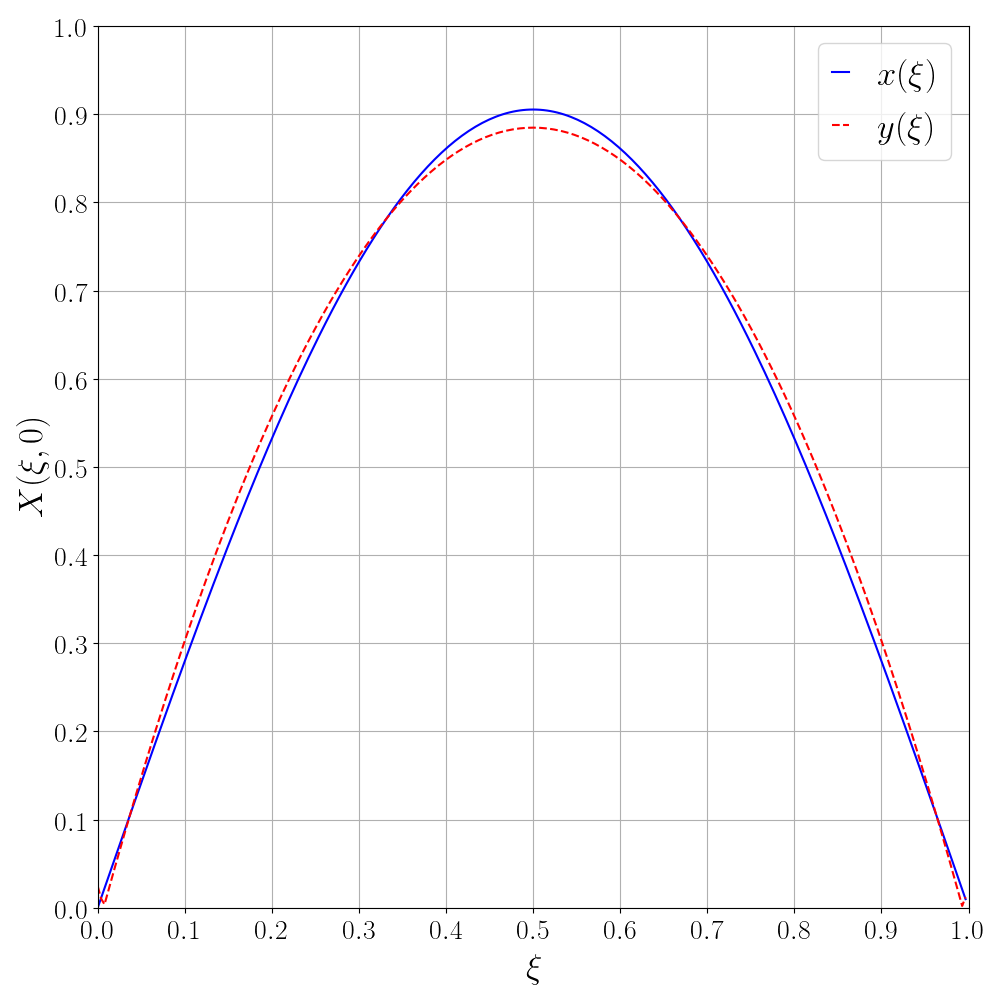
\includegraphics[width=.55\textwidth]{burgers_equation/stochastic/numerical_experiments/figures/IC.png}
		\caption{Initial condition for (\ref{burgers_stochastic2}) and its approximation.}
		\label{IC_Cheb}	
		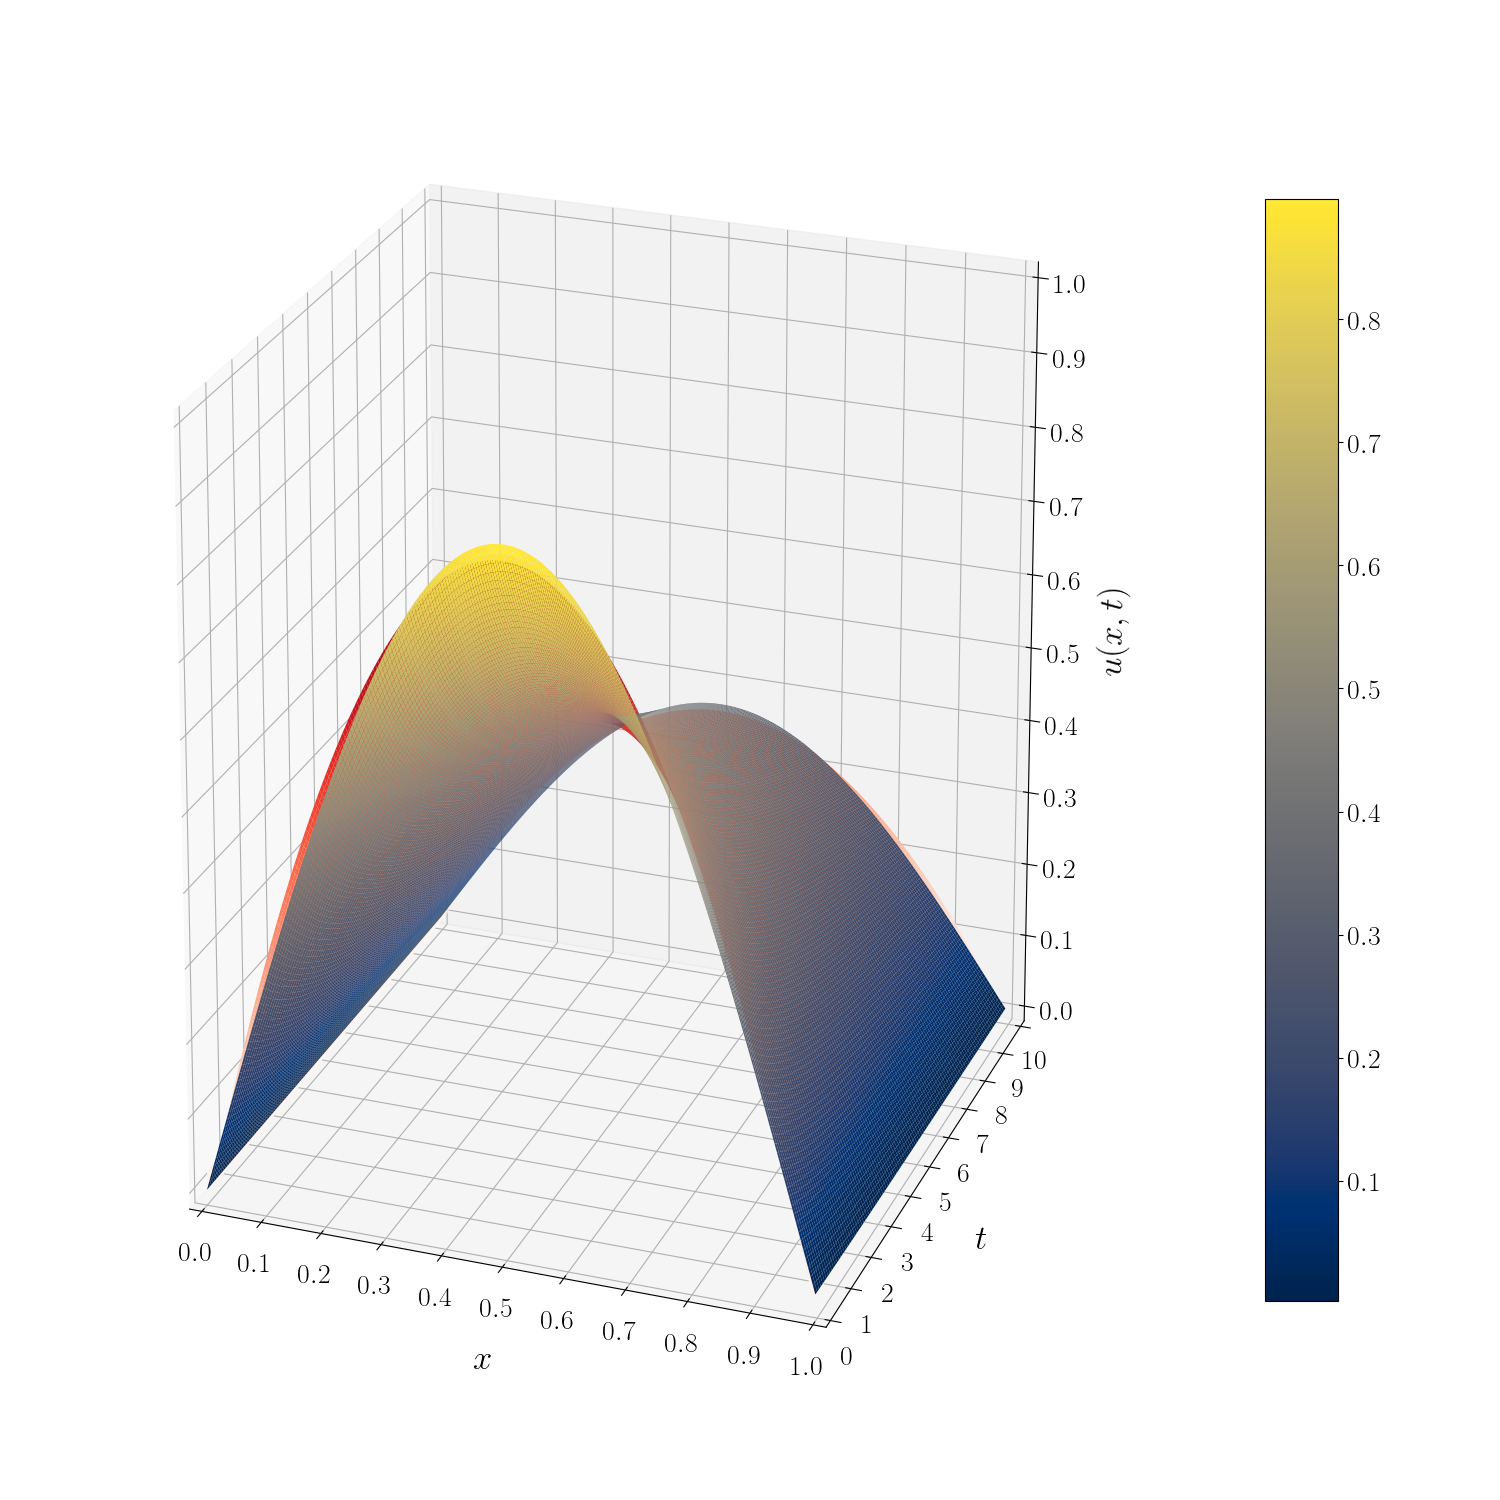
\includegraphics[width=.9\textwidth]{burgers_equation/stochastic/numerical_experiments/figures/Numerical_Solution_Stochastic.png}
		\caption{Numerical solutions for (\ref{burgers_stochastic2}) with initial conditions $x(\xi)$ and $y(\xi)$.}
		\label{Stochastic_Solutions}	
	\end{figure}
\newpage
	\begin{figure}[H]	
	\centering
		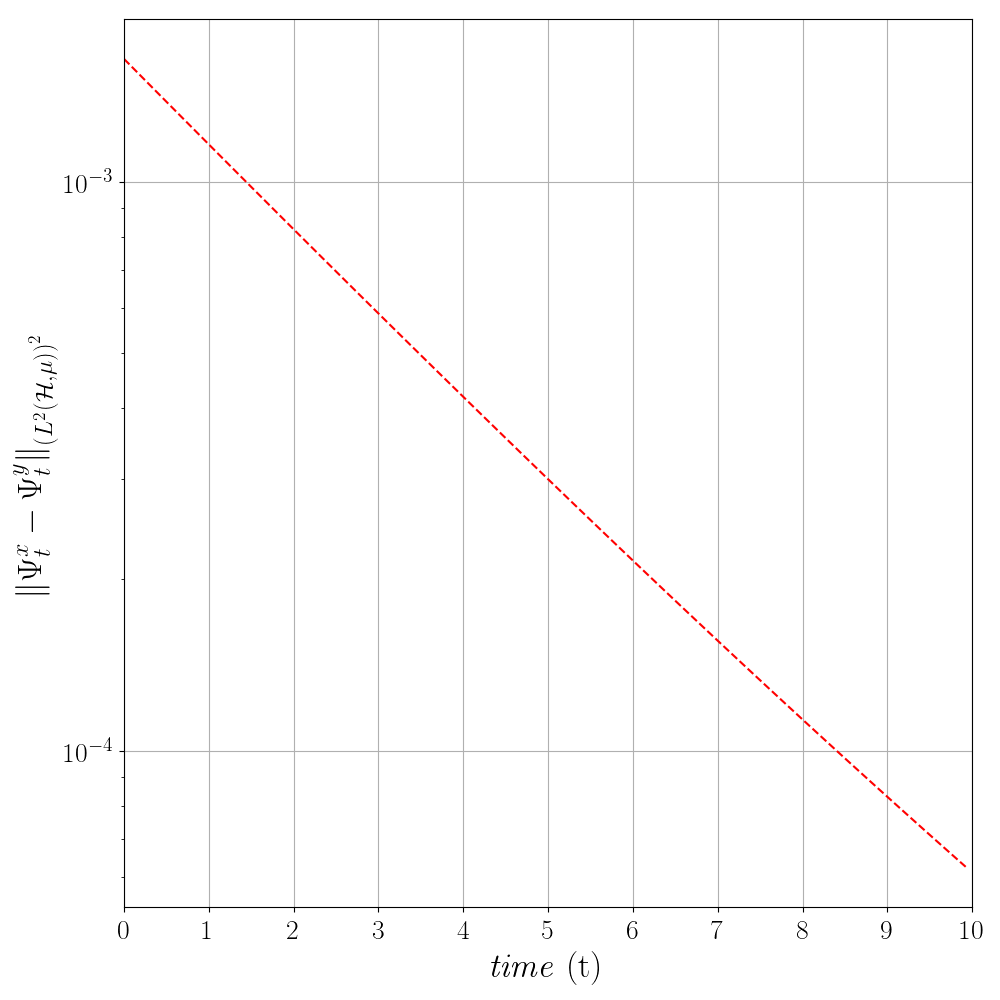
\includegraphics[width=.7\textwidth]{burgers_equation/stochastic/numerical_experiments/figures/norms.png}
		\caption{Distance between the numerical solutions for equation (\ref{burgers_stochastic2}) with initial conditions $x(\xi)$, and $y(\xi)$.}
		\label{Continuity}
	\end{figure}	
